\section{Methodology}
\label{sec:event}

In this section, we present the theoretical foundations and algorithmic formulation of \textit{{O}n-{P}olicy {D}istillation with Tail {Res}idualization} (\method{}). 
We begin in Sec.~\ref{subsec:prelim} by establishing the full-vocabulary reverse-KL gradient and analyzing the trade-off of sparse teacher payloads, exposing how naive Top-$k$ heuristics induce objective bias and why hybrid estimators like HETS suffer from tail-sampling variance. 
In Sec.~\ref{subsec:cfr}, we formulate \method{} (illustrated in Fig.~\ref{fig:framework}), demonstrating how aggregate tail masses serve as an analytic control variate to achieve an unbiased, variance-reduced estimator. 
Sec.~\ref{subsec:evidence} describes the sampling assumptions and
connects theoretical covariance bounds to observable online diagnostics and downstream task performance.
Finally, Sec.~\ref{sec:unified} extends the analysis to a two-control family.

% Finally, Sec.~\ref{subsec:evidence} outlines the evidence boundaries of our framework, connecting theoretical covariance bounds to observable online diagnostics and downstream task performance.

% We first identify the
% full-vocabulary target and the information available through sparse Teacher
% feedback (Sec.~\ref{subsec:prelim}). We then use the observable tail bucket to
% construct an unbiased residual estimator and characterize exactly when it
% reduces variance (Sec.~\ref{subsec:cfr}). Sections~\ref{subsec:implementation}
% and~\ref{subsec:evidence} describe its computation, sampling assumptions, and
% the distinction between theoretical covariance and online diagnostics.
% Sec.~\ref{sec:unified} extends the analysis to a two-control family.

\subsection{Preliminaries: From sampled gradients to an exact sparse head}
\label{subsec:prelim}

At one fixed trajectory prefix, let $p(i)>0$ and $q(i)>0$ denote Student and Teacher
next-token probabilities over a shared vocabulary $\mathcal V$. Define
\begin{equation}
 \begin{aligned}
 r_i &\coloneqq \log\frac{p_i}{q_i}, &
 \bscore_i &\coloneqq \nabla_\theta\log p_i, &
 \btoken_i &\coloneqq r_i\bscore_i.
 \end{aligned}
 \label{eq:token-gradient}
\end{equation}
Because $\sum_i p_i\bscore_i=\bm 0$, the full-vocabulary reverse-KL gradient is
\begin{equation}
 \bgrad
 =\sum_i p_i\btoken_i
 =\E_{A\sim p}\!\left[\btoken_A\right].
 \label{eq:full-gradient}
\end{equation}
Here, $\btoken_A$ denotes the stopped-coefficient sampled-token OPD gradient. Equation~(\ref{eq:full-gradient}) demonstrates that this sampled-token gradient is an unbiased estimator of the full-vocabulary reverse-KL gradient.

\paragraph{Why direct Teacher Top-$k$ rKL is biased.}
Let $S$ be the fixed Teacher Top-$k$ support, with $0<k<|\mathcal V|$, $P=\sum_{i\in S}p_i$ and
$Q=\sum_{i\in S}q_i$. Two common scalar shortcuts have different biases:
\begin{equation}
 L_{\mathrm{renormalized}}
 =\KL\!\left(\frac{p_S}{P}\middle\|\frac{q_S}{Q}\right),
 \qquad
 L_{\mathrm{truncated}}=\sum_{i\in S}p_i\log\frac{p_i}{q_i}.
 \label{eq:topk-shortcuts}
\end{equation}
Renormalization depends only on the conditional distribution within $S$. And for every omitted logit $z_j$, $\partial L_{\mathrm{renormalized}}/\partial z_j=0$. Truncation retains the unnormalized head but introduces a boundary term:
\begin{equation}
 \frac{\partial L_{\mathrm{truncated}}}{\partial z_j}
 =-p_j\underbrace{\sum_{i\in S}p_i(r_i+1)}_{C_S},
 \qquad j\notin S.
 \label{eq:truncated-tail-push}
\end{equation}
When $C_S>0$, gradient descent increases every omitted logit.
We adopt the stopped-coefficient alternative \citep{zhu2026many}
$\bhead=\sum_{i\in S}p_i r_i\bscore_i$ in our experiments, which avoids that scalar boundary term but is
still biased by the omitted tail. Appendix~\ref{app:topk-bias} proves all three statements.

\begin{figure}[t]
\centering
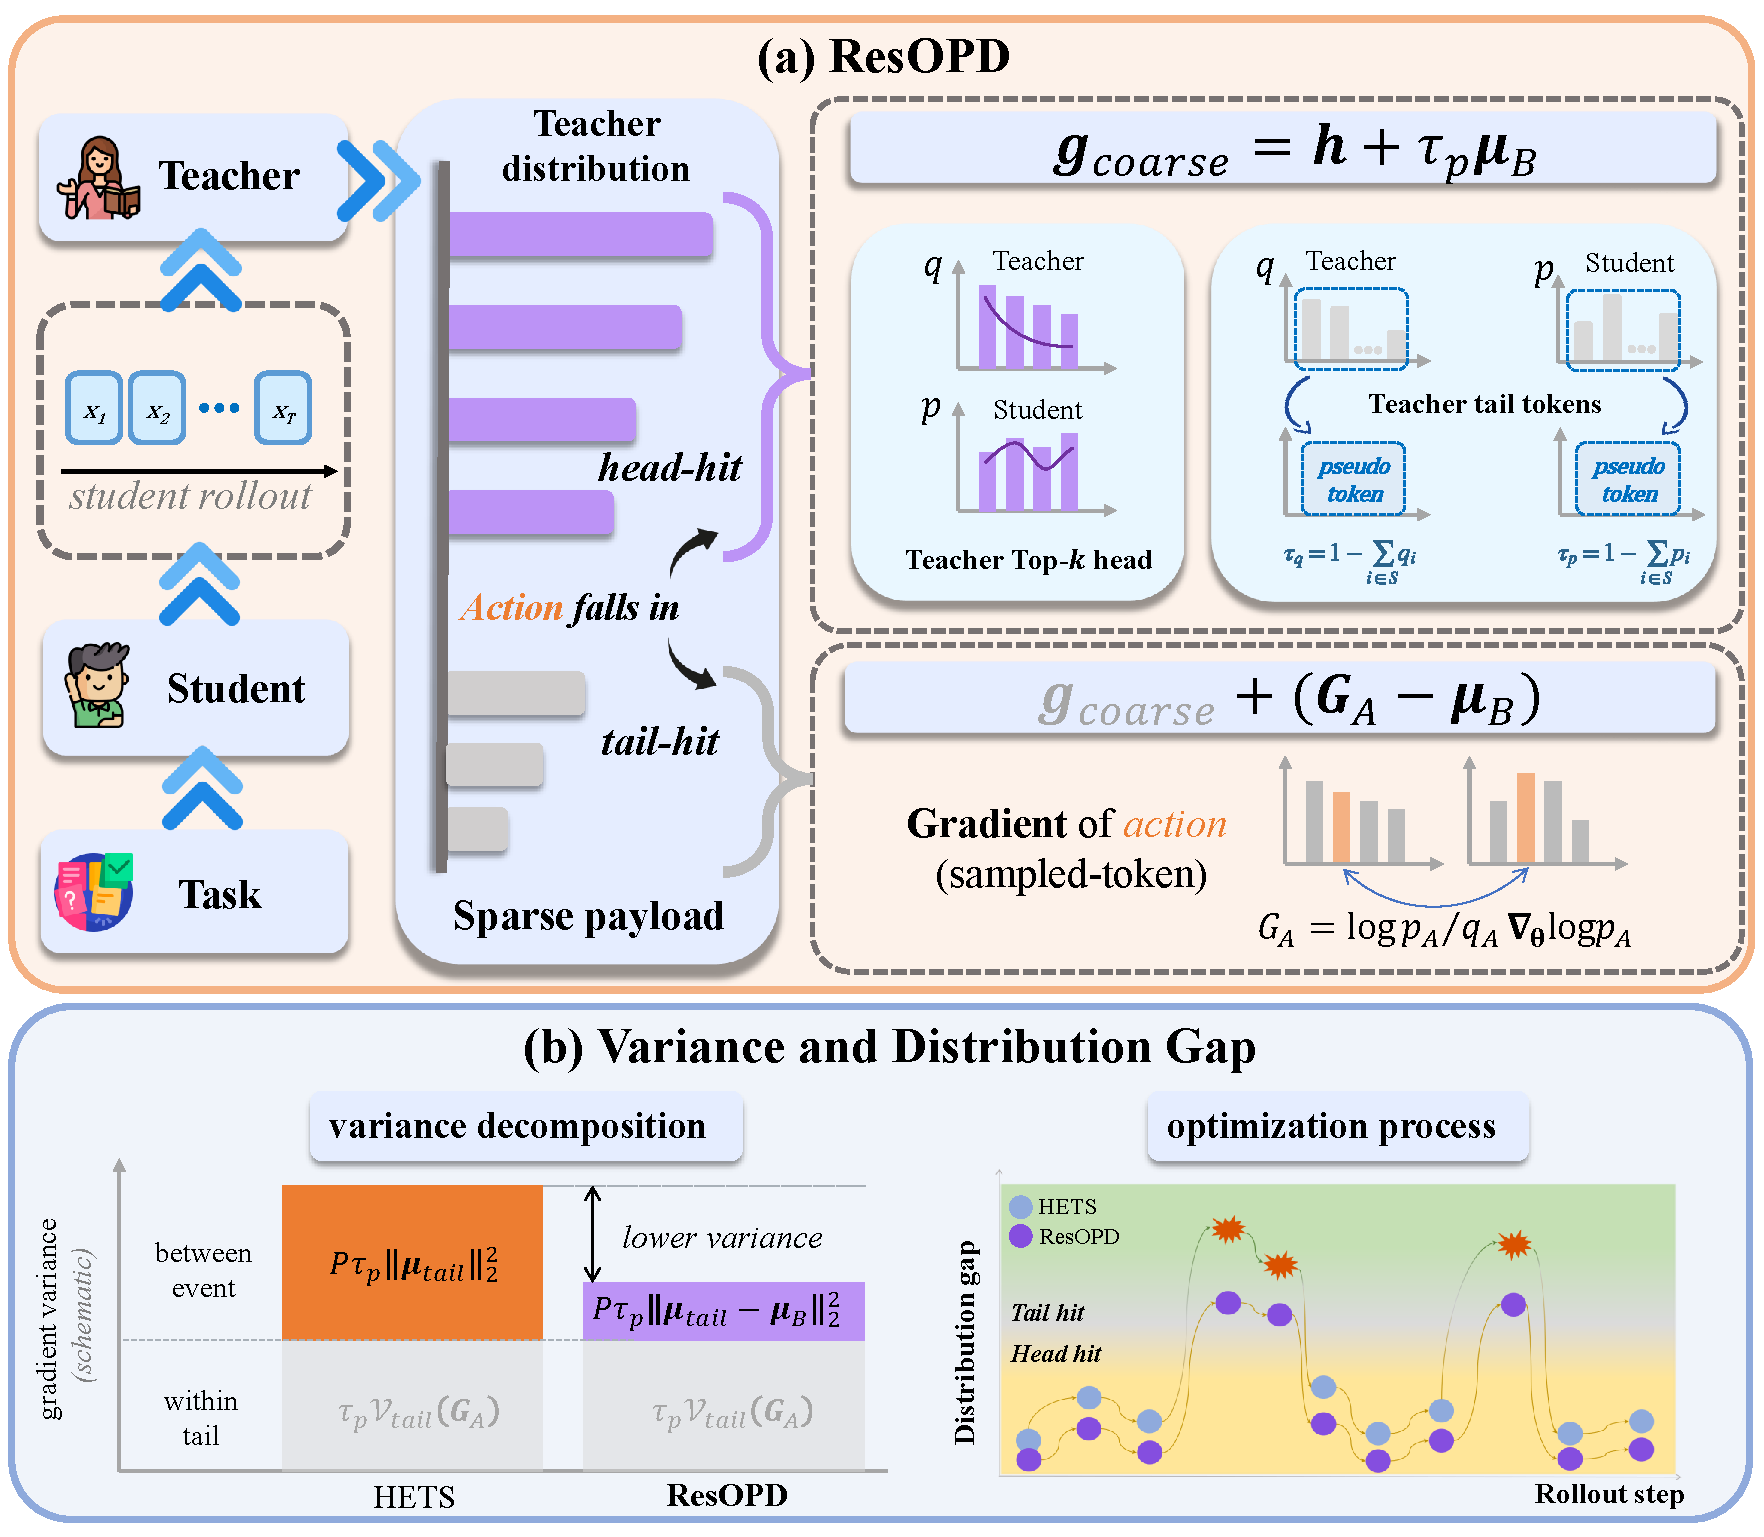
\includegraphics[width=0.8\textwidth]{figs/framework_v11.pdf}
\caption{
\textbf{Overview of ResOPD.}
(a) When the student sampled-token falls in the head, ResOPD uses only the exact coarse gradient; upon a tail hit, it adds a residual correction. (b) ResOPD suppresses between-event variance compared to HETS by centering tail samples around $\boldsymbol{\mu}_B$, achieving superior alignment with the teacher distribution across rollout steps.
}
\label{fig:framework}
\end{figure}

The interface returns full-normalized $q_i$ for $i\in S$ and $q_A$ for the
sampled action. Write
\begin{equation}
  \begin{gathered}
  \tau_p\coloneqq1-P,\qquad \tau_q\coloneqq1-Q,\\[-1pt]
  \bhead\coloneqq P\,\E[\btoken_A\mid A\in S] = \sum_{i\in S} p_i\btoken_i,
  \qquad
  \bmean_{\mathrm{tail}}\coloneqq
  \E\!\left[\btoken_A\mid A\notin S\right] = \frac{1}{\tau_p}\sum_{i\notin S} p_i\btoken_i.
  \end{gathered}
  \label{eq:head-tail-definitions}
\end{equation}
The head $\bhead$ is exactly known, while the fine-tail mean gradient is unavailable. With
$J=\ind\{A\notin S\}$, the prior Head-Exact Tail-Sampled estimator is
\begin{equation}
 \widehat{\bgrad}^{\mathrm{HETS}}
 =\bhead+J\btoken_A,
 \qquad
 \E\!\left[\widehat{\bgrad}^{\mathrm{HETS}}\right]
 =\bhead+\tau_p\bmean_{\mathrm{tail}}=\bgrad.
 \label{eq:g0}
\end{equation}
This \gzero{} baseline \citep{zhang2026ema} equals stopped Teacher Top-$k$ rKL
on head draws and adds the entire correction only on tail draws:
\begin{equation}
 \widehat{\bgrad}^{\mathrm{HETS}}
 =
 \begin{cases}
  \bhead, & A\in S,\\
  \bhead+\btoken_A, & A\notin S,
 \end{cases}
 \qquad
 \Pr(A\in S)=P.
 \label{eq:g0-rare-correction}
\end{equation}
Large $P$ therefore creates a rare-correction regime: most tokens use the
biased head-only update, while long minibatches still accumulate many sampled tail corrections.

\subsection{Tail residualization}
\label{subsec:cfr}

Top-$k$ also reveals aggregate tail masses.
Following the tail-bucketing approach in \citet{hubotter2026reinforcement} and \citet{huang2026tail}, collapsing the tail into a single pseudo-token yields
\begin{equation}
 \begin{aligned}
 b&\coloneqq\log\frac{\tau_p}{\tau_q}, &
 \bar{\bscore}_{\mathrm{tail}}
 &\coloneqq\E[\bscore_A\mid J=1]
   =\nabla_\theta\log\tau_p, &
 \bmean_B&\coloneqq b\,\bar{\bscore}_{\mathrm{tail}}.
 \end{aligned}
 \label{eq:bucket-vector}
\end{equation}
The exact gradient of the resulting complete coarse distribution is
\begin{equation}
 \bgrad_{\mathrm{coarse}}
 =\bhead+\tau_p\bmean_B.
 \label{eq:coarse-gradient}
\end{equation}
Here $\bmean_B$ predicts, but need not equal, the unavailable fine-tail mean. In fact, this formulation can be generalized to arbitrary baseline vectors: for $A\sim p$ and any prefix-dependent baseline vector $\bcontrol$,
\begin{equation}
\widehat{\bgrad}(\bcontrol)=\bhead+\tau_p\bcontrol+J(\btoken_A-\bcontrol),
\label{eq:residualization}
\end{equation}
is unbiased, i.e., $\E_{A\sim p}\!\left[\widehat{\bgrad}(\bcontrol)\right]=\bgrad$. Fig.~\ref{fig:framework} summarizes the construction.
HETS is the special case $\bcontrol=\bm0$. The expectation is explicit:
\begin{equation}
 \E[\widehat{\bgrad}(\bcontrol)]
 =\bhead+\tau_p\bcontrol
  +\tau_p(\bmean_{\mathrm{tail}}-\bcontrol)
 =\bgrad.
 \label{eq:residualization-expectation}
\end{equation}
The control may depend on the fixed prefix and current model probabilities,
but must be fixed with respect to the sampled action and stopped before
backward.
Furthermore, defining the total variance of any random vector $\bm{X}$ as $\mathcal{V}(\bm{X}) \coloneqq \operatorname{tr}(\operatorname{Cov}(\bm{X}))$, applying the law of total covariance yields the explicit variance of $\widehat{\bgrad}(\bm B)$:
\begin{equation}
\mathcal{V}(\widehat{\bgrad}(\bm B)) = \tau_p\mathcal{V}_{\mathrm{tail}}(\btoken_A)
+ P\tau_p\lVert\bmean_{\mathrm{tail}}-\bm B\rVert_2^2,
\label{eq:single-control-variance-1}
\end{equation}
where $\mathcal{V}_{\mathrm{tail}}(\btoken_A) \coloneqq \operatorname{tr}(\operatorname{Cov}(\btoken_A \mid A \in \mathrm{tail}))$.
Here, the first term $\tau_p\mathcal{V}_{\mathrm{tail}}(\btoken_A)$ captures the baseline-invariant within-tail sampling variance (weighted by the tail probability $\tau_p$), while the second term accounts for the between-event variance induced by the residual approximation error $\lVert\bmean_{\mathrm{tail}}-\bm B\rVert_2^2$, scaled by \(P\tau_p\), the variance of the binary head-versus-tail indicator.
To see this directly, condition on $J$: the head branch is deterministic,
the tail branch retains $\Cov_{\mathrm{tail}}(\btoken_A)$, and the two
conditional means differ by $\bmean_{\mathrm{tail}}-\bm B$. The law of total
covariance then gives Equation~(\ref{eq:single-control-variance-1}).

Equation~(\ref{eq:single-control-variance-1}) also shows that the variance of the estimator $\widehat{\bgrad}(\bcontrol)$ is minimized when the control vector is set to the true tail mean, i.e., $\bcontrol = \bmean_{\mathrm{tail}}$. However, since $\bmean_{\mathrm{tail}}$ is unavailable in practice, ResOPD substitutes it with the computable tail-bucket surrogate $\bmean_B$:
\begin{equation}
\widehat{\bgrad}^{\mathrm{ResOPD}}
=\bgrad_{\mathrm{coarse}}+J(\btoken_A-\bmean_B).
\label{eq:event}
\end{equation}

The predictable coarse correction now appears on every draw; only the
fine-tail residual remains rare.
ResOPD achieves strictly lower variance than HETS whenever $\lVert\bmean_{\mathrm{tail}}-\bmean_B\rVert_2 < \lVert\bmean_{\mathrm{tail}}\rVert_2$, i.e., whenever the tail-bucket vector $\bmean_B$ predicts the true tail mean better than zero, as observed in aggregate in our frozen-prefix audits. The complete derivation is given in Appendix~\ref{app:single-control}.

% \subsection{Practical computation with sparse feedback}
% \label{subsec:implementation}

% The Teacher supplies its full-normalized probabilities on $S$ and the score
% $q_A$ of the actual Student action, including when $A\notin S$. The Student
% computes $p_i$ on this support, $p_A$, and $\tau_p=1-\sum_{i\in S}p_i$
% from its full-normalized logits. Thus $\tau_q=1-\sum_{i\in S}q_i$ and
% $b=\log(\tau_p/\tau_q)$ are observable without requesting individual Teacher
% tail probabilities. Student and Teacher token IDs must refer to the same
% vocabulary.

% The tail-bucket score can also be expressed entirely through the head:
% \begin{equation}
%  \nabla_\theta\log\tau_p
%  =-\frac{1}{\tau_p}\sum_{i\in S}p_i\bscore_i.
%  \label{eq:bucket-head-computation}
% \end{equation}
% Consequently, neither the exact coarse gradient nor the sampled residual
% requires an additional Teacher forward pass. Sparsity reduces Teacher
% communication; the Student still computes its full-vocabulary normalization.

% For clarity, an equivalent stopped-coefficient scalar surrogate is
% \begin{equation}
%  \begin{aligned}
%  L_{\mathrm{sur}}
%  &=\sum_{i\in S}\operatorname{stopgrad}(p_i r_i)\log p_i
%    +\operatorname{stopgrad}(\tau_p b)\log\tau_p\\
%  &\quad+J\left[
%       \operatorname{stopgrad}(r_A)\log p_A
%       -\operatorname{stopgrad}(b)\log\tau_p
%     \right].
%  \end{aligned}
%  \label{eq:resopd-surrogate}
% \end{equation}
% Differentiating this expression gives exactly
% Equation~(\ref{eq:event}). Its scalar value is a gradient surrogate, rather
% than a deterministic full reverse-KL objective. In a token-level training
% implementation, prompt and padding positions are masked before aggregation.

\subsection{Sampling assumptions and evidence boundaries}
\label{subsec:evidence}

The unbiasedness identities above assume $A\sim p_\theta$ at the fixed prefix.
% with the same full-normalized Student distribution used in the gradient.
Rollout filters change this sampling law. Our primary mathematics experiments (Sec.~\ref{sec:math-opd}) use
temperature $1.0$, rollout top-$p=0.95$, and rollout top-$k=20$, while the
full-support audits (Sec.~\ref{sec:exact-audit}) and cross-domain runs (Sec.~\ref{sec:cross-domain}) use the ancestral condition. Sec.~\ref{sec:ex-setup} specifies both, and
Sec.~\ref{sec:rollout-ablation} evaluates the effect of removing the filters.

The coarse-to-fine variance decomposition can also be characterized
under an arbitrary realized rollout distribution $\tilde p$. Let
$\tilde{\tau}=\Pr_{\tilde p}(A\notin S)$ and
$\tilde{\bm\mu}_{\mathrm{tail}}
=\mathbb{E}_{\tilde p}[\bm G_A\mid A\notin S]$.
For
$\hat{\bm g}(\bm B)=\bm h+\tau_p\bm B+
\mathbb{I}\{A\notin S\}(\bm G_A-\bm B)$,
the estimator still admits the exact decomposition
\begin{equation}
\mathcal V_{\tilde p}(\hat{\bm g}(\bm B))
=
\tilde{\tau}\mathcal V_{\tilde p,\mathrm{tail}}(\bm G_A)
+
(1-\tilde{\tau})\tilde{\tau}
\|\tilde{\bm\mu}_{\mathrm{tail}}-\bm B\|_2^2 .
\label{eq:realized-rollout-variance}
\end{equation}
Hence, for $0<\tilde{\tau}<1$, ResOPD has strictly lower sampling variance than HETS
whenever
$\|\tilde{\bm\mu}_{\mathrm{tail}}-\bm\mu_B\|_2
<\|\tilde{\bm\mu}_{\mathrm{tail}}\|_2$.
The expected update under this realized sampling law is
\begin{equation}
 \E_{\tilde p}[\widehat{\bgrad}(\bm B)]
 =\bhead+\tau_p\bm B
  +\tilde\tau(\tilde{\bm\mu}_{\mathrm{tail}}-\bm B).
 \label{eq:realized-rollout-mean}
\end{equation}
The variance identity remains exact under $\tilde p$, but it does not turn a
truncated rollout into an unbiased draw from $p_\theta$.
Crucially, truncation is confined strictly to sequence generation. All student quantities ($p_i$, $r_i$, $s_i$, $\tau_p$, and the coarse-tail terms) are faithfully recomputed via a fresh, untruncated forward pass during training.

Equation~(\ref{eq:single-control-variance-1}) characterizes estimator quality
at fixed prefixes. We test it by exact action enumeration
(Sec.~\ref{sec:exact-audit}). During online OPD, both policies and visited
prefixes change, while sparse Teacher feedback hides the fine tail.
% We therefore monitor residual second moments $M_2$ as inexpensive diagnostics
% whose definitions and interpretation are given before the training-dynamics
% results in Sec.~\ref{sec:online-residual-moments}. These moments do not
% estimate full gradient covariance.
We instead monitor residual second moments \(M_2\) as cheap mechanism-aligned online diagnostics. Their decline is consistent with reduced head-versus-tail event noise, but does not by itself estimate full gradient covariance.
Appendix~\ref{app:online-residual-moments} gives the exact definitions.

Nevertheless, variance reduction does not imply monotonic downstream accuracy gains. Lower covariance trace reduces stochastic optimization noise, but final performance is still shaped by training dynamics and decoding randomness, both of which are discretized by benchmark scoring. Thus, ResOPD can reliably suppress gradient noise without strictly outperforming HETS at every checkpoint. We therefore view theoretical covariance, online residual moments, and downstream accuracy as complementary signals across different stages of the learning pipeline.
